\setchapterimage[4cm]{images/004_Headerchapter1.png}
\setchapterpreamble[u]{\margintoc}
\chapter{Mathematical and Physical Background}
\labch{MathAndBackground}

In this chapter I will describe the most common options used, both the 
ones inherited from \Class{scrbook} and the \Class{kao}-specific ones. 
Options passed to the class modifies its default behaviour; beware 
though that some options may lead to unexpected results\ldots

\section{Linear Algebra}

	[Introduction Linear Algebra]
	\subsection{Matrices}
		[Matrices]
	\subsection{Matrix Operation}
		[Determinant]
		[Matrix multiplication]

\section{Reference Coordinate Frames }
\subsection{Cartesian Coordinates}
\subsection{Spherical Coordinates}

\subsection{Earth Centered Inertial - ECI}

The Earth Centered Inertial - short ECI - is usually the frame of choice as inertial reference system. The point of origin is the center of the target body, with the z axis pointing to the north pole an the x axis pointing towards the point of Aries. Hence this coordinate frame is non-rotating. 
\begin{figure}[h!]
	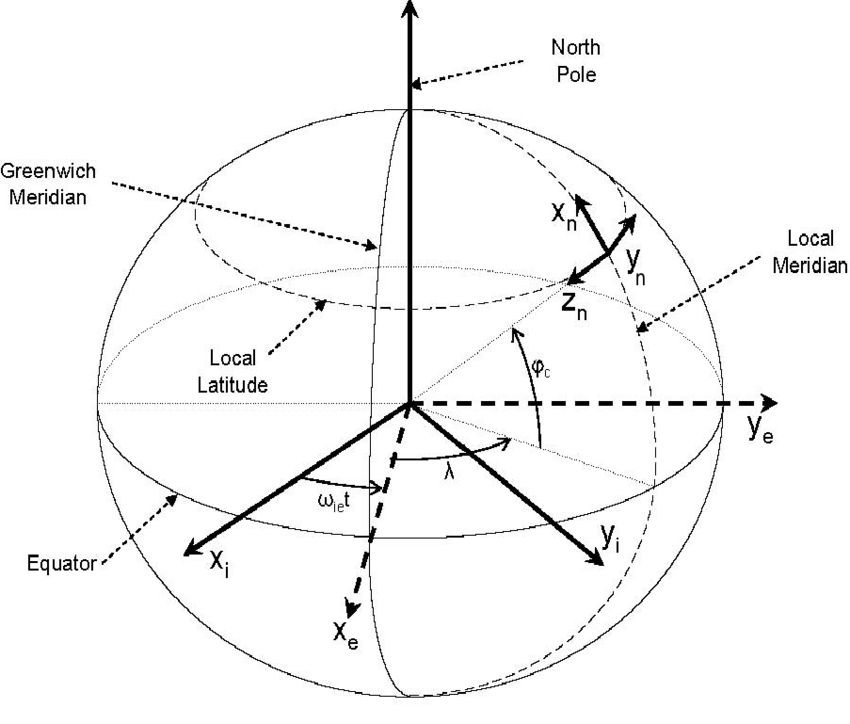
\includegraphics[width=0.6\textwidth]{001_ECI}
	\caption[Earth Centered Intertial]{Earth Centered Intertial. }
	\labfig{fig:eci}
\end{figure}

\subsection{Earth Centered Earth Fixed - ECEF}
	The Earth Centered Earth Fixed - short ECEF - coordinate frame has its point of origin at the target body's center and is rotating with the rotational period of the target body (e.g. for Earth the rotational period would be 24 hours). The z-axis is pointing towards the north pole and the x-axis towards the Greenwich Meridian (or Zero meridian). That makes ECI and ECEF almost identical systems. The only difference is the rotation around their common z-axis that is causing an angle between the zero meridian and the point of Aries. \\
	The ECEF frame is most commonly used to give the geographic position of the spacecraft with respect to the target body. Furhtermore, it is common to use spherical coordinates for this frame with the following elements: 
		\begin{itemize}
			\item Longitude
			\item Latitude 
			\item Radius or Altitude (with respect to a mean surface radius)
		\end{itemize}

\begin{figure}[h!]	
	\includegraphics[width=0.6\textwidth]{002_ECEF}
	\caption[Earth Centered Earth Fixed]{Earth Centered Earth Fixed. The spherical Coordinates Longitude $\lambda$, Latitude $\phi$ and Radius show the geographical position of the spacecraft. Less commonly used but also possible is to express the position in spherical coordinates x,y,z. }
	\labfig{fig:ecef}
\end{figure}

\begin{kaobox}[frametitle=Reference Body]
	Note that Earth Centered Inertial as well as Earth Centered Earth Fixed come inherently the strong implication that the reference body is indeed Earth. The basic principle of these coordinate frames however can be applied to any arbitrary planetary body. Since the abbreviation is quite prominent it is common to use ECI and ECEF even if the reference body is not Earth. In the context of this book ECI does not always necessarily refer to Earth.
\end{kaobox}

\subsection{North East Down - NED}
\subsection{Aerodynamic Frame - A}
\subsection{Bodyfixed Frame - B}

\section{Coordinate Frame Transformation}
	\subsection{Spherical to Cartesian Coordinates}
	\subsection{Cartesian to Spherical Coordinates}
	\subsection{ECI to ECEF}
	\subsection{B to NED}
	
	
\section{Equations of Translational Motion}

\section{Equations of Rotational Motion}

\section{External Forces}
	\subsection{Gravitational Forces}
	\subsection{Aerodynamic Forces}
